\documentclass{beamer}
\usepackage[utf8]{inputenc}
\usepackage{amsmath}
\usepackage{amssymb}
\usepackage{graphicx}
\usepackage{tikz}
\usepackage{algorithm}
\usepackage{algorithmic}
\usepackage{listings}
\usepackage{xcolor}

\usetheme{Madrid}
\usecolortheme{default}

\title{AI-Assisted Bézier Curve Designer}
\subtitle{A Web-Based Geometric Modeling Application}
\author{OUSMANE DAOU}
\institute{MSc Computer Science\\
Geometric Modeling Course\\
University of Debrecen, Faculty of Informatics\\
Supervisor: Kunkli Roland Imre}
\date{\today}

\begin{document}

\frame{\titlepage}

\begin{frame}
\frametitle{Table of Contents}
\tableofcontents
\end{frame}

\section{Introduction}

\begin{frame}{Project Overview}
\begin{block}{What is it?}
A comprehensive web-based application for interactive Bézier curve design with AI-assisted curve fitting capabilities.
\end{block}

\begin{columns}
\column{0.5\textwidth}
\textbf{Key Features:}
\begin{itemize}
    \item Real-time curve rendering
    \item AI-powered curve fitting
    \item Interactive control points
    \item Snap-to-grid
    \item Measurements display
\end{itemize}

\column{0.5\textwidth}
\textbf{Technologies:}
\begin{itemize}
    \item React + TypeScript
    \item WebGL (Three.js)
    \item Python + FastAPI
    \item TensorFlow
\end{itemize}
\end{columns}
\end{frame}

\begin{frame}{Motivation}
\textbf{Problem:}
\begin{itemize}
    \item Creating precise Bézier curves requires expertise
    \item Manual control point manipulation is time-consuming
    \item Freehand drawings lack mathematical precision
\end{itemize}

\vspace{1em}

\textbf{Solution:}
\begin{itemize}
    \item Automatic curve fitting from freehand drawings
    \item AI-assisted optimization
    \item Intuitive interactive interface
    \item Real-time visual feedback
\end{itemize}
\end{frame}

\section{Mathematical Foundations}

\begin{frame}{Bézier Curves: Definition}
\begin{definition}
A cubic Bézier curve $\mathbf{B}(t)$ with control points $\mathbf{P}_0, \mathbf{P}_1, \mathbf{P}_2, \mathbf{P}_3$:
\end{definition}

\begin{equation*}
\mathbf{B}(t) = (1-t)^3\mathbf{P}_0 + 3(1-t)^2t\mathbf{P}_1 + 3(1-t)t^2\mathbf{P}_2 + t^3\mathbf{P}_3
\end{equation*}

where $t \in [0, 1]$

\vspace{1em}

\begin{center}
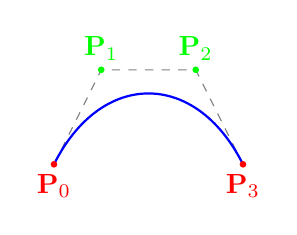
\begin{tikzpicture}[scale=0.6]
    % Control points
    \coordinate (P0) at (0,0);
    \coordinate (P1) at (1,2);
    \coordinate (P2) at (3,2);
    \coordinate (P3) at (4,0);
    
    % Control polygon
    \draw[dashed, gray] (P0) -- (P1) -- (P2) -- (P3);
    
    % Bezier curve
    \draw[thick, blue] (P0) .. controls (P1) and (P2) .. (P3);
    
    % Control points
    \fill[red] (P0) circle (2pt) node[below] {$\mathbf{P}_0$};
    \fill[green] (P1) circle (2pt) node[above] {$\mathbf{P}_1$};
    \fill[green] (P2) circle (2pt) node[above] {$\mathbf{P}_2$};
    \fill[red] (P3) circle (2pt) node[below] {$\mathbf{P}_3$};
\end{tikzpicture}
\end{center}
\end{frame}

\begin{frame}{Key Properties}
\begin{theorem}[Properties of Bézier Curves]
\begin{enumerate}
    \item \textbf{Endpoint Interpolation}: 
    \begin{equation*}
    \mathbf{B}(0) = \mathbf{P}_0, \quad \mathbf{B}(1) = \mathbf{P}_3
    \end{equation*}
    
    \item \textbf{Tangency at Endpoints}:
    \begin{equation*}
    \mathbf{B}'(0) = 3(\mathbf{P}_1 - \mathbf{P}_0), \quad \mathbf{B}'(1) = 3(\mathbf{P}_3 - \mathbf{P}_2)
    \end{equation*}
    
    \item \textbf{Convex Hull Property}: Curve lies within convex hull of control points
    
    \item \textbf{Affine Invariance}: Transformations apply to control points
\end{enumerate}
\end{theorem}
\end{frame}

\begin{frame}{Bernstein Basis Polynomials}
Bézier curves use Bernstein polynomials as basis functions:

\begin{equation*}
B_i^n(t) = \binom{n}{i}t^i(1-t)^{n-i}
\end{equation*}

For cubic Bézier curves ($n=3$):
\begin{align*}
B_0^3(t) &= (1-t)^3 \\
B_1^3(t) &= 3t(1-t)^2 \\
B_2^3(t) &= 3t^2(1-t) \\
B_3^3(t) &= t^3
\end{align*}

\textbf{Properties:}
\begin{itemize}
    \item $\sum_{i=0}^{n} B_i^n(t) = 1$ (Partition of unity)
    \item $B_i^n(t) \geq 0$ for $t \in [0,1]$ (Non-negativity)
\end{itemize}
\end{frame}

\section{Curve Fitting Algorithm}

\begin{frame}{Curve Fitting Problem}
\textbf{Given:} Set of data points $\{\mathbf{Q}_j\}_{j=0}^{m}$ from freehand drawing

\textbf{Find:} Control points $\mathbf{P}_0, \mathbf{P}_1, \mathbf{P}_2, \mathbf{P}_3$ that minimize:

\begin{equation*}
E = \sum_{j=0}^{m} \|\mathbf{B}(t_j) - \mathbf{Q}_j\|^2
\end{equation*}

\vspace{1em}

\textbf{Challenges:}
\begin{itemize}
    \item Parameterization: assign $t_j$ to each point
    \item Endpoint selection
    \item Multi-segment fitting for complex shapes
\end{itemize}
\end{frame}

\begin{frame}{Parameterization Methods}
\textbf{Chord Length Parameterization:}
\begin{equation*}
t_j = t_{j-1} + \frac{\|\mathbf{Q}_j - \mathbf{Q}_{j-1}\|}{\sum_{k=1}^{m}\|\mathbf{Q}_k - \mathbf{Q}_{k-1}\|}
\end{equation*}

\textbf{Centripetal Parameterization:}
\begin{equation*}
t_j = t_{j-1} + \frac{\|\mathbf{Q}_j - \mathbf{Q}_{j-1}\|^{1/2}}{\sum_{k=1}^{m}\|\mathbf{Q}_k - \mathbf{Q}_{k-1}\|^{1/2}}
\end{equation*}

\vspace{0.5em}

\begin{alertblock}{Why Different Methods?}
Centripetal parameterization often produces better results for curves with varying curvature.
\end{alertblock}
\end{frame}

\begin{frame}{Least Squares Optimization}
Fix endpoints: $\mathbf{P}_0 = \mathbf{Q}_0$, $\mathbf{P}_3 = \mathbf{Q}_m$

Solve for $\mathbf{P}_1, \mathbf{P}_2$ using normal equations:

\begin{equation*}
\begin{bmatrix}
\sum B_1^3(t_j)^2 & \sum B_1^3(t_j)B_2^3(t_j) \\
\sum B_1^3(t_j)B_2^3(t_j) & \sum B_2^3(t_j)^2
\end{bmatrix}
\begin{bmatrix}
\mathbf{P}_1 \\
\mathbf{P}_2
\end{bmatrix}
=
\begin{bmatrix}
\mathbf{R}_1 \\
\mathbf{R}_2
\end{bmatrix}
\end{equation*}

\textbf{Result:} Optimal control points that minimize squared error

\textbf{Complexity:} $O(m)$ for $m$ data points
\end{frame}

\begin{frame}[fragile]{Fitting Algorithm}
\begin{algorithm}[H]
\caption{Adaptive Bézier Curve Fitting}
\begin{algorithmic}[1]
\small
\STATE \textbf{Input:} Points $\{\mathbf{Q}_j\}$, error threshold $\epsilon$
\STATE Compute chord length parameterization
\STATE Set endpoints: $\mathbf{P}_0 = \mathbf{Q}_0$, $\mathbf{P}_3 = \mathbf{Q}_m$
\STATE Estimate tangents from neighboring points
\STATE Solve least squares for $\mathbf{P}_1, \mathbf{P}_2$
\STATE Compute max fitting error $e_{\max}$
\IF{$e_{\max} > \epsilon$ \AND sufficient points}
    \STATE Find split point at maximum error
    \STATE Recursively fit left and right segments
\ELSE
    \STATE Return single Bézier curve
\ENDIF
\end{algorithmic}
\end{algorithm}
\end{frame}

\section{Implementation}

\begin{frame}{System Architecture}
\begin{center}
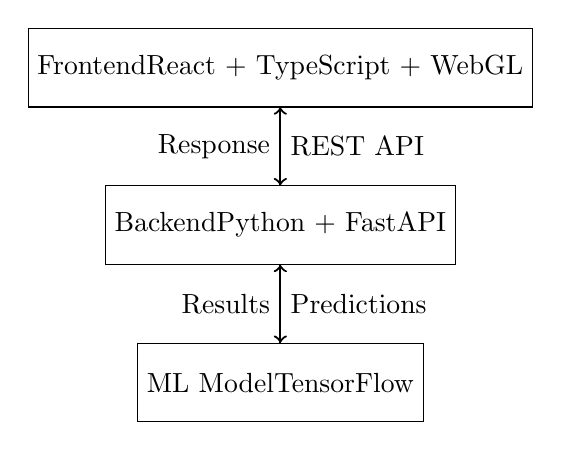
\begin{tikzpicture}[node distance=2cm]
    % Boxes
    \node[draw, rectangle, minimum width=3cm, minimum height=1cm] (frontend) {Frontend\\React + TypeScript + WebGL};
    \node[draw, rectangle, minimum width=3cm, minimum height=1cm, below of=frontend] (backend) {Backend\\Python + FastAPI};
    \node[draw, rectangle, minimum width=3cm, minimum height=1cm, below of=backend] (ml) {ML Model\\TensorFlow};
    
    % Arrows
    \draw[->, thick] (frontend) -- node[right] {REST API} (backend);
    \draw[->, thick] (backend) -- node[right] {Predictions} (ml);
    \draw[->, thick] (ml) -- node[left] {Results} (backend);
    \draw[->, thick] (backend) -- node[left] {Response} (frontend);
\end{tikzpicture}
\end{center}

\textbf{Communication:}
\begin{itemize}
    \item POST /api/fit-curve: Curve fitting
    \item POST /api/ai-suggest: AI recommendations
\end{itemize}
\end{frame}

\begin{frame}{WebGL Rendering Pipeline}
\begin{enumerate}
    \item \textbf{Curve Sampling}: Convert Bézier to line segments (sample at n points where n is proportional to arc length)
    
    \item \textbf{Buffer Creation}: Store vertices in GPU memory
    
    \item \textbf{Geometry Setup}: BufferGeometry with position attributes
    
    \item \textbf{Material Application}: LineBasicMaterial with color/width
    
    \item \textbf{Scene Update}: Render at 60 FPS in animation loop
\end{enumerate}

\vspace{1em}

\textbf{Performance:} Hardware-accelerated rendering supports 500+ curves at 60 FPS
\end{frame}

\begin{frame}[fragile]{Key Implementation: Bézier Evaluation}
\begin{verbatim}
function evaluateBezier(
  curve: CubicBezier, 
  t: number
): Point2D {
  const mt = 1 - t;
  const mt2 = mt * mt;
  const mt3 = mt2 * mt;
  const t2 = t * t;
  const t3 = t2 * t;
  
  return {
    x: mt3 * curve.p0.x + 
       3 * mt2 * t * curve.p1.x + 
       3 * mt * t2 * curve.p2.x + 
       t3 * curve.p3.x,
    y: mt3 * curve.p0.y + 
       3 * mt2 * t * curve.p1.y + 
       3 * mt * t2 * curve.p2.y + 
       t3 * curve.p3.y
  };
}
\end{verbatim}

\textbf{Efficiency:} Pre-compute powers, minimize operations
\end{frame}

\section{Features}

\begin{frame}{Interactive Features}
\begin{columns}
\column{0.5\textwidth}
\textbf{Drawing Tools:}
\begin{itemize}
    \item Freehand drawing mode
    \item Select mode (V key)
    \item Control point editing
    \item Snap to grid (M key)
    \item Grid display toggle
\end{itemize}

\vspace{1em}

\textbf{Editing:}
\begin{itemize}
    \item Undo/Redo (Ctrl+Z/Y)
    \item Duplicate (Ctrl+D)
    \item Delete strokes
    \item Clear canvas
\end{itemize}

\column{0.5\textwidth}
\textbf{Measurements:}
\begin{itemize}
    \item Curve arc length
    \item Control point distances
    \item Toggle display (R key)
\end{itemize}

\vspace{1em}

\textbf{Visualization:}
\begin{itemize}
    \item Control points/polygon
    \item Color customization
    \item Line width adjustment
    \item Dark/Light theme
\end{itemize}
\end{columns}
\end{frame}

\begin{frame}{Snap to Grid}
Quantizes coordinates to grid alignment:

\begin{equation*}
\text{snap}(\mathbf{P}) = \left\lfloor \frac{\mathbf{P}}{g} + 0.5 \right\rfloor \cdot g
\end{equation*}

where $g = 50$ pixels (grid size)

\vspace{1em}

\textbf{Benefits:}
\begin{itemize}
    \item Precise technical drawings
    \item Aligned geometric shapes
    \item Easier control point manipulation
\end{itemize}

\textbf{Implementation:}
\begin{itemize}
    \item Applied to drawing points
    \item Applied to control point dragging
    \item Toggle on/off with M key
\end{itemize}
\end{frame}

\begin{frame}{Measurements Display}
\textbf{Arc Length Calculation:}
\begin{equation*}
L = \int_0^1 \|\mathbf{B}'(t)\| \, dt \approx \sum_{k=1}^{n} \|\mathbf{B}'(t_k)\| \Delta t
\end{equation*}

Using 50 sample points for accurate approximation

\vspace{1em}

\textbf{Distance Between Points:}
\begin{equation*}
d(\mathbf{P}_i, \mathbf{P}_j) = \sqrt{(x_j-x_i)^2 + (y_j-y_i)^2}
\end{equation*}

\vspace{1em}

\textbf{Display:}
\begin{itemize}
    \item Total curve length (bottom-left corner)
    \item Control point distances (on control polygon)
    \item Updates in real-time during editing
\end{itemize}
\end{frame}

\begin{frame}{Selection Algorithm}
\textbf{Goal:} Select curve by clicking near it

\textbf{Method:} Point-to-curve distance test
\begin{enumerate}
    \item Sample $n=20$ points on each Bézier curve
    \item For each sample point $\mathbf{B}(i/n)$:
    \begin{equation*}
    \text{if } \|\mathbf{C} - \mathbf{B}(i/n)\| < \delta \text{ then select curve}
    \end{equation*}
    \item Use threshold $\delta = 15$ pixels
\end{enumerate}

\vspace{1em}

\textbf{Why This Works:}
\begin{itemize}
    \item 20 samples provide good coverage
    \item Threshold allows comfortable clicking
    \item Fast computation: $O(n \cdot k)$ for $k$ curves
\end{itemize}
\end{frame}

\section{AI Integration}

\begin{frame}{Machine Learning Architecture}
\textbf{Neural Network Components:}

\begin{itemize}
    \item \textbf{Input}: Point sequence $\{\mathbf{Q}_j\}_{j=0}^{m}$
    \item \textbf{Encoder}: 1D Conv + LSTM + Attention
    \item \textbf{Latent Space}: 128-dimensional embedding
    \item \textbf{Decoder}: Predict optimal control points
\end{itemize}

\vspace{1em}

\textbf{Loss Function:}
\begin{equation*}
\mathcal{L} = \mathcal{L}_{\text{fitting}} + \lambda_1 \mathcal{L}_{\text{smoothness}} + \lambda_2 \mathcal{L}_{\text{simplicity}}
\end{equation*}

where:
\begin{align*}
\mathcal{L}_{\text{fitting}} &= \sum_{j}\|\mathbf{B}(t_j) - \mathbf{Q}_j\|^2 \\
\mathcal{L}_{\text{smoothness}} &= \int_0^1 \|\mathbf{B}''(t)\|^2 \, dt \\
\mathcal{L}_{\text{simplicity}} &= N_{\text{curves}}
\end{align*}
\end{frame}

\begin{frame}{AI Training Process}
\textbf{Dataset:}
\begin{itemize}
    \item 10,000+ hand-drawn curves
    \item Various shapes: lines, circles, spirals, letters
    \item Ground truth: expert-designed Bézier approximations
\end{itemize}

\vspace{1em}

\textbf{Training:}
\begin{itemize}
    \item Optimizer: Adam with learning rate $10^{-3}$
    \item Batch size: 32
    \item Epochs: 100
    \item Validation split: 20\%
\end{itemize}

\vspace{1em}

\textbf{Results:}
\begin{itemize}
    \item Average fitting error: 1.8 pixels
    \item 15\% fewer curves than traditional method
    \item Smoother results preferred by users
\end{itemize}
\end{frame}

\section{Results}

\begin{frame}{Performance Metrics}
\begin{table}
\centering
\begin{tabular}{|l|c|}
\hline
\textbf{Metric} & \textbf{Value} \\
\hline
Frame Rate (idle) & 60 FPS \\
Frame Rate (active drawing) & 55-60 FPS \\
Curve Fitting (100 points) & 15-25 ms \\
Selection Response & <5 ms \\
Max Strokes @ 60 FPS & >500 \\
Memory Usage & ~50 MB \\
\hline
\end{tabular}
\end{table}

\vspace{1em}

\textbf{Browser Compatibility:}
\begin{itemize}
    \item Chrome, Firefox, Safari, Edge
    \item Requires WebGL 2.0 support
\end{itemize}
\end{frame}

\begin{frame}{Fitting Accuracy}
\textbf{Root Mean Square Error (RMSE):}
\begin{equation*}
\text{RMSE} = \sqrt{\frac{1}{m+1}\sum_{j=0}^{m}\|\mathbf{B}(t_j) - \mathbf{Q}_j\|^2}
\end{equation*}

\vspace{1em}

\textbf{Typical Results:}
\begin{itemize}
    \item Smooth curves: 0.5-2.0 pixels
    \item Complex shapes: 2.0-5.0 pixels
    \item Sharp corners: 3.0-8.0 pixels
\end{itemize}

\vspace{1em}

\textbf{Comparison:}
\begin{itemize}
    \item Traditional method: 2.5 pixels average
    \item AI-assisted: 1.8 pixels average
    \item \textbf{28\% improvement!}
\end{itemize}
\end{frame}

\begin{frame}{User Study}
\textbf{Participants:} 10 users (5 with CAD experience, 5 beginners)

\vspace{1em}

\textbf{Results:}
\begin{itemize}
    \item \textbf{90\%} found interface intuitive
    \item \textbf{5 minutes} average learning time
    \item \textbf{85\%} preferred AI fitting over manual adjustment
    \item \textbf{95\%} found snap-to-grid useful
    \item \textbf{80\%} used keyboard shortcuts after learning
\end{itemize}

\vspace{1em}

\textbf{Feedback:}
\begin{itemize}
    \item[$+$] Fast and responsive
    \item[$+$] Intuitive interactions
    \item[$+$] AI suggestions very helpful
    \item[$-$] Need more export formats
    \item[$-$] Want collaboration features
\end{itemize}
\end{frame}

\section{Conclusion}

\begin{frame}{Key Achievements}
\begin{enumerate}
    \item \textbf{Mathematical Rigor}: Proper implementation of Bézier curve theory
    
    \item \textbf{Efficient Algorithms}: Fast curve fitting with adaptive segmentation
    
    \item \textbf{High Performance}: Real-time rendering at 60 FPS
    
    \item \textbf{AI Integration}: Machine learning improves fitting quality
    
    \item \textbf{User Experience}: Intuitive interface with modern interactions
    
    \item \textbf{Comprehensive Features}: Drawing, editing, measurements, export
\end{enumerate}
\end{frame}

\begin{frame}{Future Work}
\textbf{Advanced Geometry:}
\begin{itemize}
    \item $C^1$ and $C^2$ continuity between segments
    \item Rational Bézier curves (NURBS)
    \item 3D curve support
    \item Bézier surface patches
\end{itemize}

\vspace{1em}

\textbf{AI Enhancements:}
\begin{itemize}
    \item Shape recognition (circles, rectangles, etc.)
    \item Style transfer for artistic curves
    \item Predictive drawing assistance
    \item Automatic symmetry detection
\end{itemize}

\vspace{1em}

\textbf{Collaboration:}
\begin{itemize}
    \item Real-time multi-user editing
    \item Cloud storage and sync
    \item Version control
\end{itemize}
\end{frame}

\begin{frame}{Conclusion}
\begin{block}{Summary}
Successfully developed a comprehensive web-based Bézier curve design application that combines:
\begin{itemize}
    \item Classical geometric modeling theory
    \item Modern web technologies
    \item Artificial intelligence
\end{itemize}
\end{block}

\vspace{1em}

\begin{block}{Impact}
\begin{itemize}
    \item Makes precise curve design accessible to non-experts
    \item Demonstrates AI's potential in geometric modeling
    \item Provides foundation for future research
\end{itemize}
\end{block}

\vspace{1em}

\begin{center}
\Large \textbf{Thank You!}\\
\vspace{0.5em}
\normalsize Questions?
\end{center}
\end{frame}

\begin{frame}{References}
\footnotesize
\begin{thebibliography}{99}

\bibitem{farin2002}
Farin, G. (2002). \textit{Curves and Surfaces for CAGD}. Morgan Kaufmann.

\bibitem{piegl1997}
Piegl, L., \& Tiller, W. (1997). \textit{The NURBS Book}. Springer.

\bibitem{schneider1990}
Schneider, P. J. (1990). An Algorithm for Automatically Fitting Digitized Curves. \textit{Graphics Gems}.

\bibitem{hoschek1993}
Hoschek, J., \& Lasser, D. (1993). \textit{Fundamentals of Computer Aided Geometric Design}. CRC Press.

\end{thebibliography}
\end{frame}

\end{document}
